\documentclass[a4paper,english,12pt]{article}
\usepackage{%
	amsfonts,%
	amsmath,%	
	amssymb,%
	amsthm,%
	algorithm,%
	babel,%
	bbm,%
	etex,%
	%biblatex,%
	caption,%
	centernot,%
	color,%
	dsfont,%
	enumerate,%
	epsfig,%
	epstopdf,%
	geometry,%
	graphicx,%
	hyperref,%
	latexsym,%
	mathtools,%
	multicol,%
	pgf,%
	pgfplots,%
	pgfplotstable,%
	pgfpages,%
	proof,%
	psfrag,%
	subfigure,%	
	tikz,%
	ulem,%
	url%
}	
\usepackage[noend]{algpseudocode}
\usepackage[mathscr]{eucal}
\usepgflibrary{shapes}
\usetikzlibrary{%
  	arrows,%
	backgrounds,%
	chains,%
	decorations.pathmorphing,% /pgf/decoration/random steps | erste Graphik
	decorations.text,%
	matrix,%
  	positioning,% wg. " of "
  	fit,%
	patterns,%
  	petri,%
	plotmarks,%
  	scopes,%
	shadows,%
  	shapes.misc,% wg. rounded rectangle
  	shapes.arrows,%
	shapes.callouts,%
  	shapes%
}

\theoremstyle{plain}
\newtheorem{thm}{Theorem}[section]
\newtheorem{lem}[thm]{Lemma}
\newtheorem{prop}[thm]{Proposition}
\newtheorem{cor}[thm]{Corollary}

\theoremstyle{definition}
\newtheorem{defn}[thm]{Definition}
\newtheorem{conj}[thm]{Conjecture}
\newtheorem{exmp}[thm]{Example}
\newtheorem{assum}[thm]{Assumptions}
\newtheorem{axiom}[thm]{Axiom}

\theoremstyle{remark}
\newtheorem{rem}{Remark}
\newtheorem{note}{Note}
\newtheorem{fact}{Fact}

\newcommand{\norm}[1]{\left\lVert#1\right\rVert}
\newcommand{\indep}{\!\perp\!\!\!\perp}
\DeclarePairedDelimiter\abs{\lvert}{\rvert}%
\newcommand\numberthis{\addtocounter{equation}{1}\tag{\theequation}}
\newcommand{\tr}{\operatorname{tr}}
\newcommand{\R}{\mathbb{R}}
\newcommand{\N}{\mathbb{N}}
\newcommand{\E}{\mathbb{E}}
\newcommand{\Z}{\mathbb{Z}}
\newcommand{\B}{\mathscr{B}}
\newcommand{\C}{\mathcal{C}}
\newcommand{\T}{\mathscr{T}}
\newcommand{\F}{\mathcal{F}}
\newcommand{\G}{\mathcal{G}}
%\newcommand{\ba}{\begin{align*}}
%\newcommand{\ea}{\end{align*}}
\DeclareMathOperator*{\argmax}{arg\,max}
\renewcommand{\qedsymbol}{$\blacksquare$}
\makeatletter
\def\BState{\State\hskip-\ALG@thistlm}
\makeatother

\makeatletter
\def\th@plain{%
  \thm@notefont{}% same as heading font
  \itshape % body font
}
\def\th@definition{%
  \thm@notefont{}% same as heading font
  \normalfont % body font
}
\makeatother
\date{}

\pgfmathdeclarefunction{gauss}{2}{%
  \pgfmathparse{1/(#2*sqrt(2*pi))*exp(-((x-#1)^2)/(2*#2^2))}%
}

%opening
\title{Lecture 2: Minimax Hypothesis Testing}
\date{14 Jan 2016}

\begin{document}
\maketitle
\section{Continued from the Lecture 1}
At the onset, we will look into two examples of Bayesian Hypothesis Testing.
\begin{exmp}[The Binary Channel] 
A binary channel is the most common communication channel model used in coding theory and information theory. In this model, a transmitter sends a bit ($0$ or $1$), and the receiver receives it. The bit may be received correctly, or it may be "flipped" with some probability. The probability with which a flipped bit is received is known as "crossover probability". 
\par Consider transmission of a bit over such a Binary Channe. Let the observation at the output of the channel be $Y$, which can be either $0$, or $1$. Let the crossover probability be $\lambda_0$ when bit $0$ is transmitted, i.e., a transmitted $0$ is received as $1$ with probability $\lambda_0$ and as $0$ with probability (1 - $\lambda_0$), where $0 \leq \lambda_0 \leq 1$. Similarly, let the crossover probability when a $1$ is transmitted  be $\lambda_1$. A Binary Symmetric Channel (BSC) is a special case, where $\lambda_0=\lambda_1=\lambda$. Observing $Y$ does not tell us exactly whether the transmitted digit was bit $0$ or $1$. The goal is to find an optimum decision rule using the Bayesian Hypothesis Testing.
\begin{figure}[h]
\centering
\begin{tikzpicture}[scale=4]				
\draw (-0.05,0) node {${\bf 1}$} (0,0) -- (1,0) (1.05,0) node {${\bf 1}$}
node [below,midway,sloped] (TextNode) {$1-\lambda_1$};
\draw (-0.05,0.5) node {${\bf 0}$} (0,0.5) -- (1,0.5) (1.05,0.5) node {${\bf 0}$} node [above,midway,sloped] (TextNode) {$1-\lambda_0$};    
\draw (0,0) -- (1,0.5) node [pos=0.8,below] (TextNode) {$\lambda_1$} ;    
\draw (0,0.5) -- (1,0) node [pos=0.8,above] (TextNode) {$\lambda_0$} ;    
\end{tikzpicture}
\caption{Block diagram for Binary Channel}
\label{fig:bsc1}
\end{figure}
\par The two hypothesis $H_0$, and $H_1$ depic the transmission of bit $0$ and $1$ respectively. The observation set is $\Gamma=\{0,1\}$. The recieved signal $y \in \Gamma$ is an instance of a Bernoulli random variable $Y$ with probability mass funtion (pmf) dependent on the transmitted bit,
\begin{eqnarray}
Y_{0}~\sim~\mathcal{B}\left( 1-\lambda_{0}\right) ~\mbox{if}~H_0~\mbox{is transmitted},\\\nonumber
Y_{1}~\sim~\mathcal{B}\left( 1-\lambda_{1}\right)~\mbox{if}~H_1~\mbox{is transmitted},
\end{eqnarray}
where the notation $\mathcal{B}(\lambda)$ denotes the pmf of a Bernoulli random variable $p$ with parameter $\lambda$. The pmf of the observation $Y$ can be written compactly as,
\begin{equation}
p_{j}\left( y\right) =\begin{cases}
 \lambda_{j} ,\hspace{42pt}\mbox{if}~y\neq j,\\
 \left( 1-\lambda_{j}\right),\hspace{10pt}\mbox{if}~ y=j,
\end{cases}
\hspace{10pt}j \in \{0,1\}.
\end{equation}
The corresponding likelihood ratio is,
\begin{equation}
L(y) = \frac{p_1(y)}{p_0(y)} = 
\begin{cases}
	\frac{\lambda_1}{1-\lambda_0} ~~~~~~~\mbox{if}~ y=0, \\
	 \frac{1-\lambda_1}{\lambda_0} ~~~~~~~\mbox{if}~ y=1.
\end{cases}
\end{equation}
As discussed in last lecture, a Bayesian decision rule has the form,
\begin{equation}
\delta_B(y)=\mathbbm{1}_{\{L(y)\geq \tau\}},
\end{equation}
where $\tau= \frac{\pi_0(C_{10}-C_{00})}{\pi_1(C_{01}-C_{11})}$ is a threshold, which depends on the prior probability $\pi_0$ and the costs. If $\lambda_0,~\lambda_1,~\tau$  are such that $\lambda_1\geq \tau\left( 1-\lambda_0\right) $, then according to the likelihood ratio, a recieved $0$ is decided as transmitted $1$. Similarly a received $1$ is decided as a transmitted $0$ when $(1-\lambda_1)<\tau \lambda_0$.
\par Consider the simple case of uniform cost, for which, $C_{ij} = 0~ \mbox{if}~ i=j$ and $C_{ij} = 1~ \mbox{if} ~i\neq j$, and equal priors i.e.,  $\pi_0=1/2$. In this case, $\tau=1$, and the Bayesian decision rule is given as,
\begin{eqnarray}
\delta_{B}(0)=
\begin{cases}
1~\mbox{if}~(1-\lambda_1)<\lambda_0,\\ 
0~\mbox{if}~(1-\lambda_1)\geq\lambda_0,
\end{cases}\\ \nonumber
\delta_{B}(1)=\begin{cases}
1~\mbox{if}~(1-\lambda_1)\geq\lambda_0,\\
0~\mbox{if}~(1-\lambda_1)<\lambda_0.
\end{cases}
\end{eqnarray}
This can be written in a compact form as,
\begin{equation}
\delta_{B}(y)=\begin{cases}
y,\hspace{35pt}\mbox{if}~(1-\lambda_1)\geq\lambda_0\\
\left( 1-y\right), ~\mbox{if}~(1-\lambda_1)<\lambda_0.
\end{cases}
\end{equation}
For a BSC with $(\lambda_1=\lambda_0=\lambda)$,
\begin{equation}
\delta_{B}(y)=\begin{cases}
y,\hspace{35pt}\mbox{if}~\lambda\leq  0.5\\
\left( 1-y\right), ~\mbox{if}~\lambda>0.5.
\end{cases}
\end{equation}
For the optimal bayes rule descibed above, conditional risks have the following expressions,
\begin{equation}
R_0(\delta)=\begin{cases}
\lambda_0~~~~~~~~~~~\mbox{if}~(1-\lambda_1)\geq\lambda_0, \\
\left(1-\lambda_0\right)~~~\mbox{if}~(1-\lambda_1)<\lambda_0,
\end{cases}
\end{equation}
and,
\begin{equation}
R_1(\delta)=\begin{cases}
\lambda_1~~~~~~~~~~~\mbox{if}~(1-\lambda_1)\geq\lambda_0, \\
\left( 1-\lambda_1\right)~~~\mbox{if}~(1-\lambda_1)<\lambda_0.
\end{cases}
\end{equation}
The unconditional risk can be obtained as a weighted sum of the conditional risks. For a BSC, the expression for unconditional risk can be simplified to,
\begin{equation}
r(\delta)= \min\left( \lambda,1-\lambda\right).
\end{equation}
\end{exmp}
\begin{exmp}[Location Testing with Gaussian Error] 
Consider the typical communication model denoted by the equation, 
\begin{equation}
y=x+n,
\end{equation}
where $n$ is a white noise signal with mean zero, and variance $\sigma^2$.
\begin{figure}[h]
\centering
\begin{tikzpicture}
[node distance = 15mm,text height=1.2ex,text depth=.25ex, % align text horizontally 
draw=black,very thick,
point/.style={coordinate},>=latex,bend angle=20,
adder/.style={draw,circle},
block/.style={draw, rectangle, align = center, text width=7mm, inner sep = 2pt,minimum size = 7mm,very thick},
eblock/.style={rectangle, text width = 25mm, inner sep = 0pt,minimum size = 7mm,very thick},
pre/.style={<-, thick},
post/.style={->, thick},
prepost/.style={<->, double, thick},
line/.style ={draw, -latex'}
]	
\node[eblock] (e0) at (0,2) {$x\in \{\mu_0,\mu_1\}$};
\node[eblock] (e2) at (3.2,0) {$n\sim \mathcal{N}(0,\sigma^2)$};
\node[eblock] (e3) at (6,2) {$y=x+n$};
\node[adder] (e1) [right=of e0]{$+$}
    edge[pre] (e0) edge[pre] (e2) edge[post] (e3);
\end{tikzpicture}
\caption[awgn]{AWGN channel}
\label{fig:AWGN}
\end{figure}
The null hypothesis $(H_0)$ corresponds to the reception of a signal $y$ with mean $\mu_0$ and under alternative Hypothesis $(H_1)$, $y$ has mean $\mu_1$. 
\begin{eqnarray}
{H_0}~:Y \sim \mathcal{N} \left( \mu _0, \sigma^2\right), \\
{H_1}~:Y \sim \mathcal{N} \left( \mu _1, \sigma^2\right).
\end{eqnarray}
The corresponding observation space is $\Gamma = \mathcal{R}$. Assuming $\mu_1>\mu_0$, we have the following expression for the likelihood ratio $L(y)$,
\begin{align}\label{eqn:ll1}
\nonumber
L(y) = \frac{P_1(y)}{P_0(y)} &= \frac{{\frac{1}{{\sigma \sqrt {2\pi } }}\exp[\frac{{ - {{(y - {\mu _1})}^2}}}{{2{\sigma ^2}}}]
}}{{\frac{1}{{\sigma \sqrt {2\pi } }}\exp[\frac{{ - {{(y - {\mu _0})}^2}}}{{2{\sigma ^2}}}}]
}\\\nonumber
&={\exp\left[{\frac{{ - {{(y - {\mu _1})}^2} + {{(y - {\mu _0})}^2}}}{{2{\sigma ^2}}}}\right]}\\
&=\exp\left[{\frac{{(\mu_1-\mu_0)\left( {y - \frac{{{\mu _1}+{\mu _0}}}{2}} \right)}}{{{\sigma ^2}}}}\right].
\end{align}
For uniform cost and equal priors, $\tau = 1$ and $\Gamma_1 = \left\lbrace y\in \Gamma|~{L(y)\geq1}\right\rbrace$. From eqn. (\ref{eqn:ll1}), we get, 
\begin{eqnarray}
	{\exp\left[{\frac{{({\mu _{1}} - {\mu _0})\left( {y - (\frac{{{\mu_{1}} +{\mu _0}}}{2})} \right)}}{{{\sigma ^2}}}} \right]}\geq 1,\\\nonumber
	{\frac{{({\mu _{1 }}-{\mu _0})\left( {y - (\frac{{{\mu _{1}}+{\mu _0}}}{2})} \right)}}{{{\sigma ^2}}}}\geq 0.
\end{eqnarray}
In terms of $y$, we can write the decision region as,
\begin{equation}
\Gamma _1 = \left\lbrace y\in \Gamma :~ y \ge \frac{{{\mu _1} + {\mu _0}}}{2} \right\rbrace
\end{equation}
Thus, the decision rule in this case will be
\begin{equation}
\delta(y)= \begin{cases}
1 ~ \mbox{if}~  y \ge \frac{{{\mu_1} + {\mu_0}}}{2}\\
0 ~ \mbox{if}~ y < \frac{{{\mu_1} + {\mu_0}}}{2}
\end{cases}
\end{equation}
The corresponding conditional risks are,
\begin{eqnarray}\nonumber
R_0(\delta)= P_0(\Gamma_1)
=\int\limits_{{\tau'}}^\infty  {d{P_0}(x)}
=1 - \Phi \left(\frac{{\tau'-\mu_1}}{\sigma }\right)\\
R_1(\delta)= P_1(\Gamma_0)
=\int\limits_{-\infty}^{\tau'}  {d{P_1}(x)}
=\Phi \left(\frac{{\tau'-\mu_0}}{\sigma }\right)
\end{eqnarray}
\begin{figure}[h]
\centering
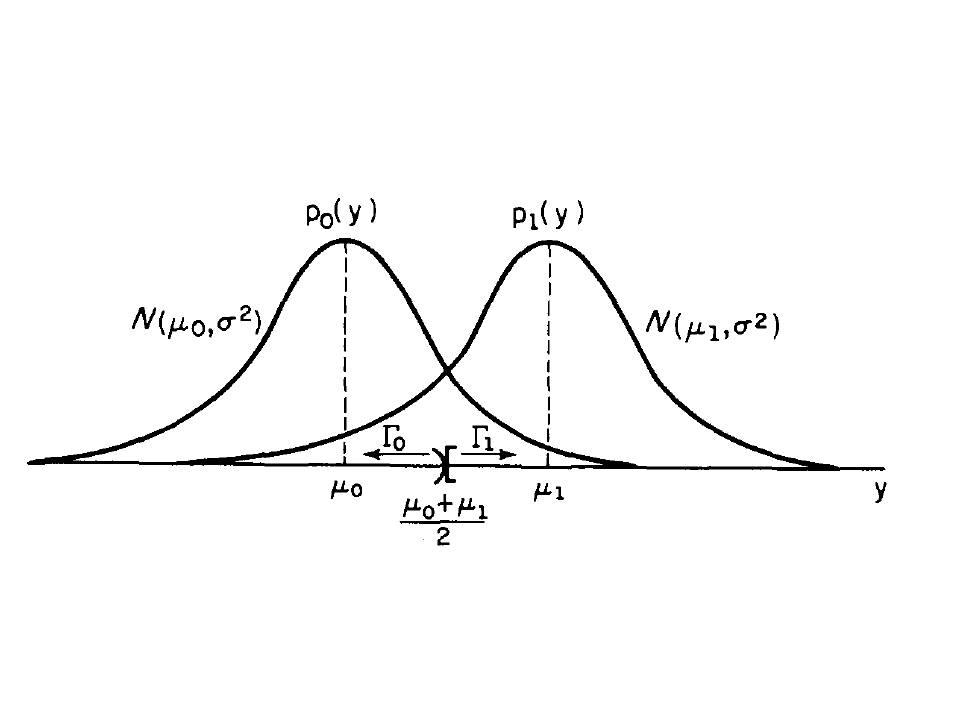
\includegraphics[trim={0 5cm 0 7cm}, width=0.9\linewidth]{Figures/gaussian_error}
\caption{Illustration of decision regions for the uniform cost and equal prior case.}
\label{fig:gaussianerror}
\end{figure}
\end{exmp}
\section{Minimax Hypothesis Testing}
Bayesian hypothesis testing assumes the knowledge of prior probabilities for the hypotheses. However, in a practical scenario, the priors are not necessarily available at the receiver. Under such circumstances, it is not possible to design a single Bayesian decision criterion that minimizes the average risk or Bayes risk for all possible prior distributions. Hence, it is necessary to develop a seperate design criterion. In this section, we look at the "Minimax criterion", which considers the minimization of the maximum of conditional risks $R_0(\delta)$ and $R_1(\delta)$ over all possible decision rules $\delta$. 
\begin{defn}
The decision rule $(\delta)$ minimising the max risk given by the expression $\max~\{R_0(\delta),R_1(\delta)\}$ is known as \textbf{Minimax Rule.}
\end{defn}
\subsection{The Minimax Rule}
\begin{figure}[h]
	\centering
	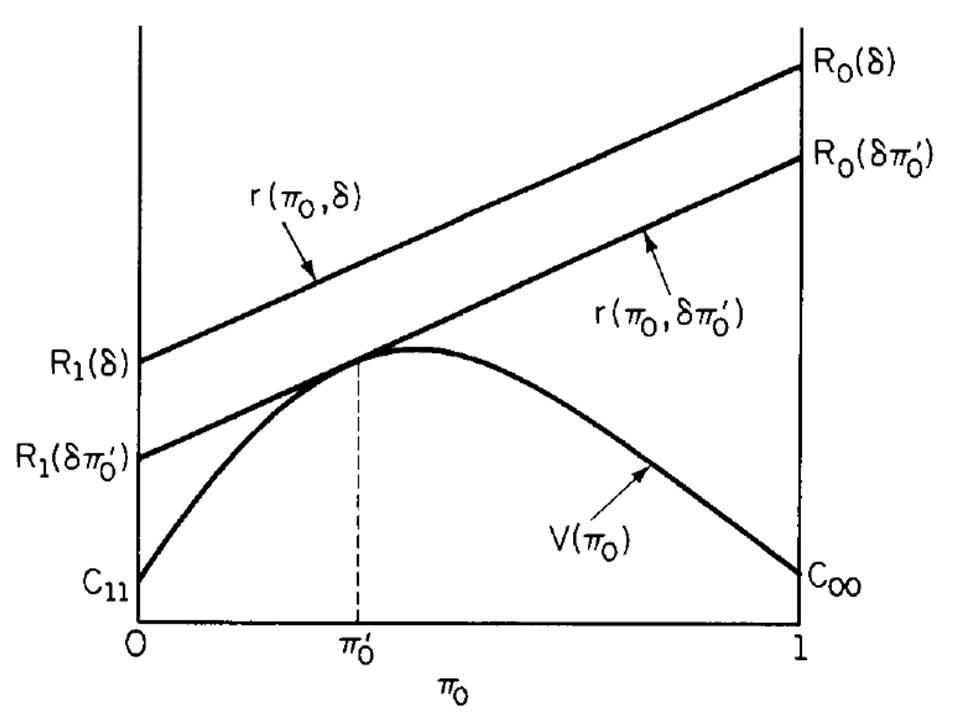
\includegraphics[width=0.9\linewidth]{Figures/minimax1}
	\caption[abc]{Illustration of the functions $r(\pi_0,\delta)~and~V(\pi_0)$}
	\label{fig:minimax1}
\end{figure}
To derive the Minimax rule, we first consider the unconditional risk for a given decision rule $\delta$ and a given prior for $H_0$, i.e $\pi_0 \in [0,1]$. The average risk for a decision rule $\delta$ is,
\begin{equation}
r(\pi_0,\delta)=~\pi_0R_0(\delta)~+~(1-\pi_0)R_1(\delta), ~~~~\pi_0 \in [0,1].
\end{equation}
The unconditional risk function is shown in Fig. \ref{fig:minimax1}. As can be seen, for a fixed $\delta$, the function $r(\pi_0,\delta)$ is a straight line taking values $R_1(\delta)~\mbox{at}~\pi_0=0$ and $R_0(\delta)~\mbox{at}~\pi_0=1$. Thus, it is an affine function, and hence attains maximum value at the extrimities,
\begin{equation}\label{eq:maxToPi}
	\mathop {\max }\limits_{0 \le {\pi _0} \le 1} r({\pi _0},\delta ) = \max\{ {R_0}(\delta ),{R_1}(\delta )\}.
\end{equation}
We can state the minimax criterion as the minimizer of the expression in eqn. (\ref{eq:maxToPi}) over all $\delta$,
\begin{equation}\label{eq:minMaxCrit}
		\mathop {\min}\limits_{\delta}\mathop {\max }\limits_{0 \le {\pi _0} \le 1} r({\pi _0},\delta ).
\end{equation}
\begin{figure}[h]
	\centering
	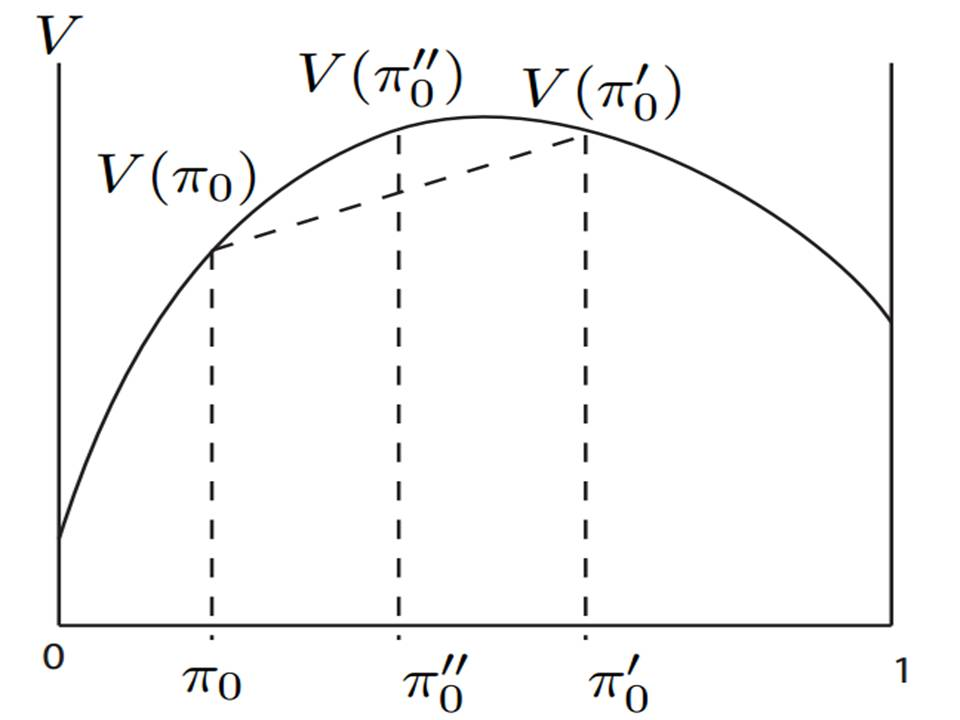
\includegraphics[width=0.7\linewidth]{Figures/concave}
	\caption{$V(\pi)$ as a concave function}
	\label{fig:concave}
\end{figure}
\par Now, for each prior $\pi_0 \in~[0,1]$, let $\delta_{\pi_0}$ denote the optimum Bayes rule corresponding to that prior, and let $V(\pi_0) = r(\pi_0,\delta_{\pi_0}) $, be the Bayes risk for the prior $\pi_0$. It can be proved that $V(\pi_0)$ is a continuous concave function of $\pi_0$ for $\pi_0 \in [0,1]$ with $V(0)=C_{11} ~and~ V(1)=C_{00}$. The proof is given below.
\begin{lem}
The function \textbf{$V(\pi):[0,1] \to\mathcal R$} is concave
\end{lem}
A function is concave, if, for any $\left\lbrace x,y\right\rbrace$ in the domain of $f$ and any $\alpha  \in [0,1],$
\begin{equation}\nonumber
f(\alpha x + (1 - \alpha )y) \ge \alpha f(x) + (1 - \alpha )f(y).
\end{equation}
\begin{proof}
Consider two priors $\pi$, $\pi'$, and a third prior $\pi''=\alpha \pi  + (1 - \alpha )\pi'$. We can write,
\begin{align}
V(\pi'' ) &= r(\pi'',\delta_{\pi''}),\\ \nonumber
&=\alpha r(\pi,{\delta_{\pi''} }) + (1 - \alpha )r(\pi' ,{\delta_{\pi ''}}).
\end{align}
Since $V(\pi)=r(\pi,\delta_\pi)$ is the minimizer of $r(\pi,\delta)$, we get,
\begin{equation}
V(\pi'' ) \ge \alpha V(\pi ) + (1 - \alpha )V(\pi' ).
\end{equation}
Hence $V(\pi)$ is concave.
\end{proof}
\par Suppose that $V(\pi_0)$ and $r(\pi_0,\delta)$ are as depicted in Fig. \ref{fig:minimax1}. Also shown in Fig. \ref{fig:minimax1} is the line labelled $r({\pi _0},{\delta _{{\pi _0'}}})$, that is both parallel to $r({\pi _0},{\delta})$ as well as tangent to $V(\pi_0)$. For this case, $\delta$ cannot be the minimax rule because the risk line shown as $r({\pi _0},{\delta _{{\pi _0'}}})$  lies completely below $r({\pi _0},{\delta})$ and thus has a smaller maximum value. Since $r({\pi _0},{\delta _{{\pi _0'}}})$ touches $V(\pi_0)$ at $\pi_0 = \pi_0'$, $\delta _{{\pi _0'}}$ is a Bayes Rule for the prior $\pi_0'$. Since a similar tangent line can be drawn for any decision rule $\delta$, it is easily seen that only Bayes Rules can possibly be Minimax rules for Fig. \ref{fig:minimax1}.
\begin{figure}[h]
	\centering
	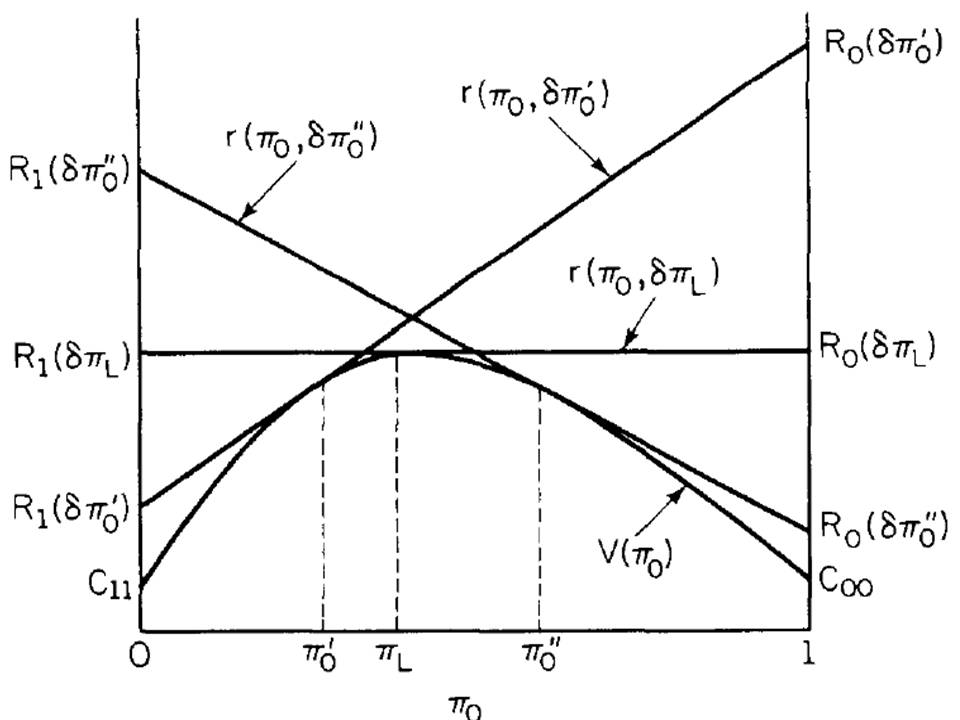
\includegraphics[width=0.7\linewidth]{Figures/minimax2}
	\caption{\textit{Illustartion of the Minimax Rule when V has an interior maximum}}
	\label{fig:minimax2}
\end{figure}
\par Moreover, by examination of Fig. \ref{fig:minimax2}, we see that the Minimax rule for this case is a Bayes rule corresponding to the prior value $\pi_L$ that maximizes $V(\pi_0)$ over $\pi_0 \in [0,1]$. Note that for this prior we have that $r(\pi_0,\delta_{\pi_L})$ is constant over $\pi_0$, so,
\begin{equation}
\max\{ {R_0}({\delta _{{\pi _L}}}),{R_1}({\delta _{{\pi _L}}})\}  = {R_0}({\delta _{{\pi _L}}}) = {R_1}({\delta _{{\pi _L}}})
\end{equation}  
The fact that $\delta_{\pi_L}$ is minimax follows from the Fig. \ref{fig:minimax2}, since if $\pi_0' < \pi_L$, we have $\max\{ {R_0}({\delta _{\pi_0'}}),{R_1}({\delta _{\pi_0'}})\}  = {R_0}({\delta _{{\pi _0'}}})>{R_0}({\delta _{{\pi _L}}})$, and if $\pi_0'' > \pi_L$, we have that
$\max\{ {R_0}({\delta _{\pi_0''}}),{R_1}({\delta _{\pi_0''}})\}  = {R_1}({\delta _{{\pi _0''}}})>{R_1}({\delta _{{\pi _L}}})$, as depicted.
Because $\pi_L$ maximizes the minimum Bayes risk, it is also called the \textbf{least-favourable prior}. Hence, a minimax decision rule is the Bayes rule for the least-favourable prior.
\begin{prop}
Suppose $\pi_L$ maximises $V(\pi_0)$ for $\pi_0 \in [0,1]$. Suppose that either $\pi_L=0$, $\pi_L=1$, or $R_1(\delta_{\pi_L})=R_0(\delta_{\pi_L})$. Then $\delta_{\pi_L}$ is a Minimax rule.
\end{prop} 
\begin{proof}
Consider the case when $R_1(\delta_{\pi_L})=R_0(\delta_{\pi_L})$. We know that, 
\begin{equation}
V(\pi_L)=\mathop {\max }\limits_{{\pi _0} \in [0,1]} \mathop {\min }\limits_\delta  r({\pi _0},\delta ) = r({\pi _L},{\delta _{{\pi _L}}})=r({\pi _0},{\delta _{{\pi _L}}}).
\end{equation}
The second equality follows from the fact that $r(\pi_0,\delta_{\pi_L})$ is a constant in $\pi_0$.
\begin{align}\label{eqn:rl}
\mathop {\max }\limits_{{\pi _0} \in [0,1]} \mathop {\min }\limits_\delta  r({\pi _0},\delta ) &= \mathop {\max }\limits_{{\pi _0} \in [0,1]} r({\pi _0},{\delta _{{\pi _L}}}), \\\nonumber
&\ge \mathop {\min }\limits_\delta  \mathop {\max }\limits_{{\pi _0} \in [0,1]} r({\pi _0},\delta ).
\end{align}
For every $\delta$, we note that,
\begin{equation}
\mathop {\max }\limits_{{\pi _0} \in [0,1]} r({\pi _0},\delta ) \ge \mathop {\max }\limits_{{\pi _0} \in [0,1]} \mathop {\min }\limits_\delta  r({\pi _0},\delta ).
\end{equation}
which shows that,
\begin{equation}\label{eqn:lr}
\mathop {\min }\limits_{\delta} \mathop {\max }\limits_{{\pi _0} \in [0,1]} r({\pi _0},\delta ) \ge \mathop {\max }\limits_{{\pi _0} \in [0,1]} \mathop {\min }\limits_\delta  r({\pi _0},\delta ).
\end{equation}
Combining eqns. (\ref{eqn:rl}), (\ref{eqn:lr}), we see that,
\begin{equation}
\mathop {\min }\limits_{\delta} \mathop {\max }\limits_{{\pi _0} \in [0,1]} r({\pi _0},\delta ) = \mathop {\max }\limits_{{\pi _0} \in [0,1]} \mathop {\min }\limits_\delta  r({\pi _0},\delta ).
\end{equation}
Indeed we have shown that, 
\begin{equation}
r({\pi _L},{\delta _{{\pi _L}}}) = \mathop {\min }\limits_\delta  \mathop {\max }\limits_{{\pi _0} \in [0,1]} r(\pi ,\delta ),
\end{equation}
which was to be shown.
\par For $\pi_L=0$, we note that, $\mathop {\max }\limits_{{\pi _0} \in [0,1]} r(\pi_0,\delta_{\pi_L})=R_1(\delta_{\pi_L})=r(\pi_L,\delta_{\pi_L})$. Using a similar argument as above, we can note that $\delta_{\pi_L}$ is a minimax rule. Similar argument can be made for $\pi_L=1$ case. This completes the proof.
\end{proof}
Now, for any $\pi_0' \in [0,1]$, $r(\pi,\delta_{\pi_0'})\geq V(\pi)$ since $V(\pi)$ minimizes Bayes risk for all $\delta$. Also $r(\pi,\delta_{\pi_0'})$ is a straight line tangent to V at $\pi=\pi_0'$. Hence, if V is differentiable,
\begin{align}
V'(\pi_0') &= \frac{d}{{d\pi }}r(\pi ,{\delta _{{\pi _0'}}})\left| {_{\pi  = {\pi _0'}}}, \right.\\\nonumber
&= {R_0}({\delta_{{\pi_0'}}})- {R_1}({\delta_{{\pi_0'}}}).
\end{align} 
If $V$ has an interior maximum, i.e., $\pi_L\in (0,1)$, then $V'(\pi_L)$ equals zero, if $V$ is differentiable at $\pi_L$. 
\par Thus, under the condition of unknown priors, Minimax rule considers the worst case scenario by taking the least favourable prior $\pi_L$ into account and minimizes the maximum unconditional risk for that prior.
\end{document}